\documentclass[svgnames,14pt]{beamer}
\usepackage{caption}
\usepackage{graphicx}
\usepackage{xcolor}
\usepackage{wrapfig}
\title{Genomes Comparision via de Bruijn graphs}
\author{Student: Ilya Minkin \\ Advisor: Son Pham}
\institute{St. Petersburg Academic University}
\setbeamertemplate{footline}[frame number]
\setbeamertemplate{navigation symbols}{}
\setbeamertemplate{caption}[numbered]
\begin{document}
\def\braces#1{[#1]}
\newenvironment{changemargin}[2]{% 
  \begin{list}{}{% 
    \setlength{\topsep}{0pt}% 
    \setlength{\leftmargin}{#1}% 
    \setlength{\rightmargin}{#2}% 
    \setlength{\listparindent}{\parindent}% 
    \setlength{\itemindent}{\parindent}% 
    \setlength{\parsep}{\parskip}% 
  }% 
  \item[]}{\end{list}}
\maketitle

\begin{frame}
\frametitle{Synteny Blocks: Algorithmic challenge}
\begin{itemize}
\item Suppose that we are given two genomes
\item The question is: how are they evolutionary related to each other?
\item In order to do rearrangements analysis we must decompose genomes into synteny blocks
\item Synteny blocks are evolutionary conserved segments of the genome
\item These blocks cover most of the genome
\item Occur in both genomes with possible variations
\end{itemize}
\end{frame}

\begin{frame}
\frametitle{Academic Project}
Project: Identify synteny blocks for duplicated genomes represented as sequences of \textbf{nucleotides}.
\begin{itemize}
\item \textbf{None} of the previous synteny blocks reconstruction software (DRIMM-Synteny (Pham And Pevzner 2010) included) can 
efficiently solve this problem. 
\item DRIMM-Synteny can find the synteny blocks for complicated genomes. But:
\pause \item It requires the genome to be represented as sequence of genes. 
\end{itemize}
\end{frame}

\begin{frame}
\frametitle{General Idea: de Bruijn Graph}
\begin{itemize}
\item We are given an alphabet \( \Sigma \) and a string \( S \) over it, \(|\Sigma| = m \)
\item A substring \( T, \, |T| = k \) is called \textit{k-mer}
\item De Bruijn graph is a multigraph \( G_{k} = (V, E) \), where \\
\( V = \Sigma^{k - 1} = \) \{all possible \( (k - 1) \)-mers\} \\
\item If \(k\)-mer \( T \) is presented in \( S \), then we add an oriented edge \( (T[1, k - 1], T[2, k]) \) to the graph
\item Create de Bruijn graph from the nucleotide sequence
\item Conserved regions will yield non-branching paths
\end{itemize}
\end{frame}

\begin{frame}
\frametitle{Challenges}
\begin{itemize}
\item Variations in synteny blocks generate cycles, so we need to simplify the graph
\item Double strandness: conserved regions may occur on both strands. Example: \\
5' \textcolor{Green}{AACC}GGTT 3' \\
3' TTGG\textcolor{Green}{CCAA} 5' \\
Such blocks are reverse complementary to each other \( \Rightarrow \) no non-branching paths
\item Spurious similarity
\item Memory efficiency
\end{itemize}
\end{frame}

\begin{frame}
\frametitle{Colored graph}
\begin{itemize}
\item We use colored de Bruijn graphs \\
\braces{Iqball et al., 2012} to handle double-strandness
\item Suppose that \( S^{+} \) and \( S^{-} \) are positive and negative strands of the chromosome
\item Colored de Bruijn graph  is a multigraph \( G_{k} = (V, E) \) where \( V =  \Sigma^{k - 1} \)
\item For each \(k\)-mer \(T^{+}\) in \(S^{+}\) add edge \( (T^{+}[1, k - 1], T^{+}[2, k]) \) to \( G_{k} \) and mark it \\ \textit{blue}
\item For each \(k\)-mer \(T^{-}\) in \(S^{-}\) add edge \( (T^{-}[1, k - 1], T^{-}[2, k]) \) to \( G_{k} \) and mark it \\ \textit{red}
\end{itemize}
\end{frame}

\begin{frame}
\frametitle{Edge labeling}
\begin{itemize}
\item Note that our graph is built from a string, not set of reads
\item Each walk in the graph represents a string
\item We are interested only in walks that represent substrings of the source string
\item Assign to each edge \( e \) label \( L(e) = \) position of the corresponding  \(k\)-mer on the positive strand
\item Walk  \( W = ( v_{1} \, e_{1} \, v_{2} \, e_{2} \, ... ) \) is considered valid iff: \\
1. \( e_{i} \) and \( e_{i + 1} \) are of the same color \\
2. \( | L(e_{i}) - L(e_{i + 1}) | = 1 \)
\end{itemize}
\end{frame}

\begin{frame}
\frametitle{Example}
\begin{changemargin}{-1.cm}{-1.cm}
\begin{figure}
\centering
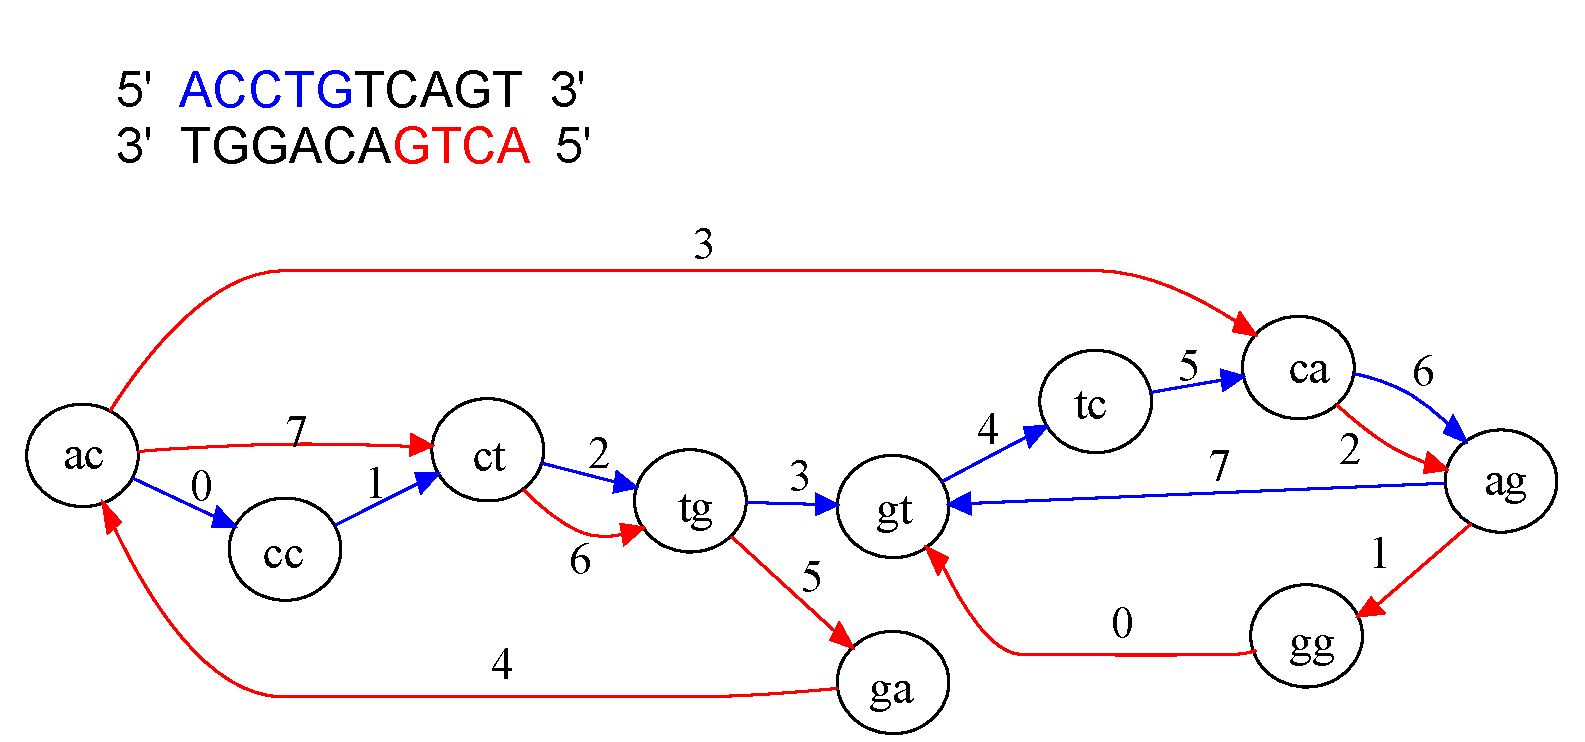
\includegraphics[scale = 0.480]{Figure1.pdf}
\small \caption{Colored de Bruijn graph built from two strands}
\end{figure}
\end{changemargin}
\end{frame}

\begin{frame}
\frametitle{Bulge removal}
\begin{itemize}
\item Bulges spoil non-brancing path
\item A pair of walks \(W_{1}, W_{2}\) is a bulge iff: \\
1) Start vertices of  \(W_{1} \) and  \(W_{2}\) are the same \\
2) End vertices of  \(W_{1} \) and  \(W_{2}\) are the same \\
3) \(W_{1} \) and  \(W_{2}\) have no common edges
\end{itemize}
\end{frame}

\begin{frame}
\frametitle{Current Progress}
Now:
\begin{itemize}
\item Program that can find absolutely conserved regions on one strand

\end{itemize}
Near future:
\begin{itemize}
\item Add graph simplification

\end{itemize}
\end{frame}

\begin{frame}
\frametitle{References}
\begin{itemize}
\item 1. Pevzner P and Tesler G, (2003) Human and mouse genomic sequences reveal extensive breakpoint reuse in mammalian evolution. 
\item 2. Pham S and Pevzner P, (2010) DRIMM-Synteny: Decomposing Genomes into Evolutionary Conserved Segments
\item 3. Iqbal Z, Caccamo M, Turner I, Flicek P, McVean G, (2012) De novo assembly and genotyping of variants using colored de Bruijn graphs
\end{itemize}
\end{frame}

\begin{center}
\hfill \huge \\
\vspace{60pt}
Thank you!
\end{center}

\end{document}
